% !TEX program = pdflatex
% 固体物理第十五次作业
\documentclass[UTF8,10pt,a4paper]{article}
\usepackage{ctex}
% \catcode`\。=\active
% \newcommand{。}{.}
\newcommand{\CourseName}{固体物理}
\newcommand{\CourseCode}{PHYS1502}
\newcommand{\Semester}{2019-2020学年第二学期}
\newcommand{\ProjectName}{第十五次作业}
\newcommand{\DueTimeType}{截止时间}
\newcommand{\DueTime}{2020. 6. 19(周五)17:00}
\newcommand{\StudentName}{陈稼霖}
\newcommand{\StudentID}{45875852}
\usepackage[vmargin=1in,hmargin=.5in]{geometry}
\usepackage{fancyhdr}
\usepackage{lastpage}
\usepackage{calc}
\pagestyle{fancy}
\fancyhf{}
\fancyhead[L]{\CourseName}
\fancyhead[C]{\ProjectName}
\fancyhead[R]{\StudentName}
\fancyfoot[R]{\thepage\ / \pageref{LastPage}}
\setlength\headheight{12pt}
\fancypagestyle{FirstPageStyle}{
    \fancyhf{}
    \fancyhead[L]{\CourseName\\
        \CourseCode\\
        \Semester}
    \fancyhead[C]{{\Huge\bfseries\ProjectName}\\
        \DueTimeType\ : \DueTime}
    \fancyhead[R]{姓名 : \makebox[\widthof{\StudentID}][s]{\StudentName}\\
        学号 : \StudentID\\
        成绩 : \underline{\makebox[\widthof{\StudentID}]{}}}
    \fancyfoot[R]{\thepage\ / \pageref{LastPage}}
    \setlength\headheight{36pt}
}
\usepackage{amsmath,amssymb,amsthm,bm}
\allowdisplaybreaks[4]
\newtheoremstyle{Problem}
{}
{}
{}
{}
{\bfseries}
{.}
{ }
{第\thmnumber{ #2}\thmname{ #1}\thmnote{ (#3)} 得分: \underline{\qquad\qquad}}
\theoremstyle{Problem}
\newtheorem{prob}{题}
\newtheoremstyle{Solution}
{}
{}
{}
{}
{\bfseries}
{:}
{ }
{\thmname{#1}}
\makeatletter
\def\@endtheorem{\qed\endtrivlist\@endpefalse}
\makeatother
\theoremstyle{Solution}
\newtheorem*{sol}{解}
\providecommand{\abs}[1]{\left\lvert#1\right\rvert}
\usepackage{graphicx}
\begin{document}
\thispagestyle{FirstPageStyle}
\begin{prob}[(21.1) Domain Walls and Geometry]
    Suppose a ferromagnet is made up of a density $\rho$ of spins each with moment $\mu_B$.
    \begin{enumerate}
        \item[(a)] Suppose a piece of this material forms a long circular rod of radius $r$ and length $L\gg r$. In zero external magnetic field, if all of the moments are aligned along the $L$-direction of the rod, calculate the magnetic energy of this ferromagnet. (Hint: a volume of aligned magnetic dipoles is equivalent to a density of magnetic monopoles on its surface.)
        \item[(b)] Suppose now the material is shaped such that $r\gg L$. What is the magnetic energy now?
        \item[(c)] If a domain wall is introduced into the material, where might it go to minimize the magnetic energy in the two different geometries. Estimate how much magnetic energy is saved by the introduction of the domain wall.
        \item[(d)] Suppose the spins in this material are arranged in a cubic lattice, and the exchange energy between nearest neighbors is denoted $J$ and the anisotropy energy is very large. How much energy does the domain wall cost? Comparing this energy to the magnetic energy, what should we conclude about which samples should have domain walls?
        \item[(e)] Note that factors of the lattice constant $a$ are often introduced in quoting exchange and anisotropy energies to make them into energies per unit length or unit volume. For magnetite, a common magnetic material, the exchange energy is $JS^2/a=1.33\times 10^{-11}$ J/m and the anisotropy energy is $\kappa S^2/a^3=1.35\times 10^4$ J/m$^3$. Estimate the width of the domain wall and its energy per unit area. \textit{Make sure you know the derivation of any formulas you use!}
    \end{enumerate}
\end{prob}
\begin{sol}
    \begin{enumerate}
        \item[(a)] 类比于两个点电荷之间电势能的公式,两个相距$r$的磁荷$q_m'$和$q_m$之间的磁能为
        \begin{align}
            E=\frac{\mu_0}{4\pi}\frac{q_mq_m'}{r}.
        \end{align}
        当长圆柱形铁磁体内部的磁矩都沿着其母线方向排列,其侧面的磁荷密度为$0$,两端均匀分布有极性相反的磁荷,磁荷密度(绝对值)等于磁矩的体密度
        \begin{align}
            \sigma_m=\mu_B\rho.
        \end{align}
        两端的磁荷量(绝对值)为
        \begin{align}
            q_m=\sigma_m\cdot A=\mu_B\rho\cdot\pi r^2.
        \end{align}
        这一铁磁体的磁能为
        \begin{align}
            E=\frac{\mu_0}{4\pi}\frac{q_m\cdot(-q_m)}{L}=-\frac{\mu_0}{4\pi}\frac{(\mu_B\rho(\pi r^2))^2}{L}.
        \end{align}
        \item[(b)] 将扁圆盘形的铁磁体材料视为储存磁荷的平行板磁容器,类比平行板电容器的电容的定义式,该平行板磁容器的磁容为
        \begin{align}
            C_m=\frac{A}{\mu_0L}=\frac{\pi r^2}{\mu_0L}.
        \end{align}
        该磁容器两极板的磁荷量仍然为
        \begin{align}
            q_m=\mu_B\rho\cdot\pi r^2.
        \end{align}
        类比平行板电容器储存电能的公式,该磁容器储存的磁能为
        \begin{align}
            E=\frac{q_m^2}{2C_m}=\frac{\mu_0(\mu_B\rho)^2(\pi r^2)L}{2}.
        \end{align}
        \item[(c)] 假设畴壁平行于圆柱体底面,则在畴壁处同性磁荷靠的很近,磁能显著增加;假设畴壁垂直于圆柱体底面,则相对于无畴壁的情况,圆柱体底面总电荷数为$0$而磁偶极矩不为$0$,两个底面之间的能量是磁偶极矩-偶极相互作用的能量,这一能量远远小于磁荷直接相互吸引的能量,因此无论是对于长圆柱体还是扁圆盘形的情况,畴壁垂直于圆柱体底面更能减小体系的能量. 对于长圆柱体的情况,能量变为
        \begin{align}
            E=\frac{\mu_0}{4\pi}\frac{(\mu_B\rho(\pi r^2/2))^2r^2}{L^3}.
        \end{align}
        对于扁圆盘形的情况,能量也有一定程度的下降,但是由于偶极矩的尺寸($\sim r$)远大于偶极矩之间的距离($\sim L$),上面能量$\sim\frac{r^6}{L^3}$的公式并不适用. 若有多个垂直于底面的畴壁,使得磁畴的尺寸$d\ll L$,则体系能量$\sim\frac{d^6}{L^3}$.
        \item[(d)] 对于长圆柱体的情况,畴壁面积为$2Lr$,畴壁上自旋面密度为$\rho^{2/3}$(对于立方晶格,晶格常数即相邻自旋的距离为$\rho^{-1/3}$,一个自旋占据的面积为$\rho^{-2/3}$),畴壁上的自旋数为$2Lr\rho^{2/3}$,故产生畴壁需要的能量为$4LrJ\rho^{2/3}$. 对于扁圆盘形的情况,假设有多个垂直于底面的畴壁,畴壁间距为$d$,则畴壁的总面积为$\frac{\pi r^2L}{d}$,畴壁上的总自旋数为$\frac{\pi r^2L}{d}$,产生这些畴壁需要的能量为$2\frac{\pi r^2LJ\rho^{2/3}}{d}$. 由于产生磁畴后,体系的磁能是$\sim L^{-6}$,而产生磁畴所需要的能量是$\sim L$,因此$L$较小的扁圆盘情况更适合产生磁畴.
        \item[(e)] 设畴壁有$N$层原子,厚度为$L=Na$. 假设自旋的方向在畴壁处均匀地由一个方向向另一个方向过渡,因此畴壁中两个相邻自旋之间的夹角为$\delta=\frac{\pi}{N}$,自旋相互作用为
        \begin{align}
            E_{one-bond}=-J\bm{S}_i\cdot\bm{S}_j=-JS^2\cos(\delta\theta)\approx-JS^2\left(1-\frac{(\delta\theta)^2}{2}+\cdots\right).
        \end{align}
        由于两个自旋之间的夹角导致的能量变化为
        \begin{align}
            \delta E_{one-bound}=JS^2(\delta\theta)^2/2=JS^2(\pi/N)^2/2.
        \end{align}
        有畴壁情况相对于无畴壁情况由于自旋相互作用导致的总能量变化为
        \begin{align}
            \frac{\delta E_{stiffness}}{A/a^2}=NJS^2(\pi/N)^2/2.
        \end{align}
        此外由于畴壁处的自旋没有沿着磁各向异性轴,相对于无畴壁情况能量变化为
        \begin{align}
            \frac{\delta E_{anisotropy}}{A/a^2}\approx\kappa S^2N.
        \end{align}
        有畴壁情况相对于无畴壁情况的能量总变化为
        \begin{align}
            \frac{\delta E_{tot}}{A/a^2}=JS^2(\pi^2/2)/N+\kappa S^2N.
        \end{align}
        为了形成畴壁,这一能量应达到最小值
        \begin{align}
            \frac{d}{dN}\frac{\delta E_{tot}}{A/a^2}=-JS^2(\pi^2/2)/N^2+\kappa S^2=0,\Longrightarrow N\sim\sqrt{J/\kappa}
        \end{align}
        代入$JS^2/a=1.33\times 10^{-11}$ J/m和$\kappa S^2/a^3=1.35\times 10^{4}$ J/m$^3$,得畴壁厚度
        \begin{align}
            L=Na=\sqrt{\frac{JS^2/s}{\kappa S^2/a^3}}=3.14\times 10^{-8}\text{m}=31.4\text{nm}.
        \end{align}
        若晶格常数$\sim 1$\AA,则差不多相当有3100层晶胞那么厚. 单位面积上磁畴的能量为
        \begin{align}
            \frac{\delta E_{tot}}{A}\sim S^2\sqrt{JK}=\sqrt{\frac{JS^2}{a}\frac{\kappa S^2}{a^3}}=4.23\times 10^{-4}\text{J/m}^2.
        \end{align}
    \end{enumerate}
\end{sol}

\begin{prob}[(21.2) Critical Field for Crytallite]
    \begin{enumerate}
        \item[(a)] Given that the energy of a crystallite in a magnetic field is given by
        \[
            E/V=E_0-\abs{M}\abs{B}\cos\theta-\kappa'\abs{M}^2(\cos\theta)^2
        \]
        show that for $\abs{B}<B_{crit}$ there is a local energy minimum where the magnetization points opposite the applied field, and find $B_{crit}$.
        \item[(b)$^*$] In part (a) we have assumed $\bm{B}$ is aligned with the anisotropy direction of the magnetization. Describe what can occur if these directions are not aligned.
        \item[(c)] For small $B$, roughly how large (in energy per unit volume) is the activation barrier for the system to get from the local minimum to the global minimum.
        \item[(d)] Can you make an estimate (in terms of actual numbers) of how big this activation barrier would be for a ferromagnetic crystal of magnetite that is a sphere of radius $1$ nm ? You may use the parameters given in Exercise 21.1.e (you may need to estimate some other parameters as well).
    \end{enumerate}
\end{prob}
\begin{sol}
    \begin{enumerate}
        \item[(a)] 设$z=\cos z$,则微晶的能量是关于$z$的开口朝下的二次函数,其对称轴为$z=-\frac{\abs{B}}{2\kappa'\abs{M}}$. 当$-\frac{\abs{B}}{2\kappa'\abs{M}}>-1$,即磁场小于临界值,$\abs{B}<B_{crit}=2\kappa'\abs{M}$时,该函数在$z\in[-1,1]$范围内有两个极小值点$z=1$和$z=1$,分别对应着$\theta=1$即磁矩与磁场同向,和$z=-1$即$\theta=\pi$磁矩与磁场反向.
        \item[(b)] 若磁场并不沿着磁各向异性方向,设磁场方向为$z$轴,各向异性轴与之成夹角$\phi$,则微晶的能量为
        \begin{align}
            E/V=E_0-\abs{M}\abs{B}\cos\theta-\kappa'\abs{M}^2\cos^2(\phi-\theta).
        \end{align}
        当磁场较强,能量表达式中第二项占主导,则极小值点$\theta\rightarrow 0$,磁极化方向趋于与磁场方向同向;当磁场较弱,能量表达式中第三项占主导,则极小值点$\theta\rightarrow\phi$或$\theta\rightarrow\pi+\pi$,磁极化方向趋向于沿着易磁化轴方向.
        \item[(c)] 对于弱磁场,微晶的能量为
        \begin{align}
            E/V\approx E_0-\kappa'\abs{M}^2\cos^2\theta.
        \end{align}
        能量极小值为$E/V(\theta=-\pi)=E_0-\kappa'\abs{M}^2$,能量极大值为$E/V(\theta=0)=E_0$,从亚稳态跨过能量极大值达到能量最小的稳定状态所需要的能量(activation barrier)为$\kappa'\abs{M}^2$.
        \item[(d)] 上一题中的anisotropy energy(单位体积中由于自旋顺着磁各向异性轴带来的能量)就是单位体积activation barrier,因此半径为$1$nm的铁磁球状晶体的activation barrier为
        \begin{align}
            \frac{\kappa S^2}{a^3}\cdot\frac{4}{3}\pi r^3=1.35\times 10^4\text{J/m}^3\times\frac{4}{3}\pi\times(10^{-9}\text{m})^3=5.65\times 10^{-23}\text{J}=0.353\text{meV}.
        \end{align}
        这个能量差不多对应着$4$K的温度.
    \end{enumerate}
\end{sol}

\begin{prob}[(22.1)$\ddagger$ Weiss Mean Field Theory of a Ferromagnet]
    Consider the spin-$1/2$ ferromagnetic Heisenberg Hamiltonian o the cubic lattice:
    \[
        \mathcal{H}=-\frac{J}{2}\sum_{\langle i,j\rangle}\bm{S}_i\cdot\bm{S}_j+g\mu_B\bm{B}\sum_i\bm{S}_i\tag{22.7}
    \]
    Here, $J>0$, with the sum indicated with $\langle i,j\rangle$ means summing over $i$ and $j$ being neighboring sites of the cubic lattice, and $\bm{B}$ is the externally applied magnetic field, which we will assume is in the $\hat{z}$ direction for simplicity. The factor of $1/2$ out front is included so that each pair of spins is counted only once. Each site $i$ is assumed to have a spin $\bm{S}_i$ of spin $S=1/2$. Here $\mu_B$ is the conventional Bohr magneton defined to be positive. The fact that the final term has a $+$ sign out front is from the fact that the electron charge is negative, therefore the magnetic moment opposes the spin direction. If one were to assume that these were nuclear spins the sign would be reversed (and the magnitude would be much smaller due to the larger nuclear mass).
    \begin{enumerate}
        \item[(a)] Focus your attention on one particular spin $\bm{S}_i$, and write down an effective Hamiltonian for this spin, treating all other variables $\bm{S}_j$ with $j\neq i$ as expectations $\langle\bm{S}_j\rangle$ rather than operators.
        \item[(b)] Calculate $\langle\bm{S}_i\rangle$ in terms of the temperature and the fixed variables $\langle\bm{S}_j\rangle$ to obtain a mean-field self-consistency equation. Write the magnetization $M=\abs{\bm{M}}$ in terms of $\langle\bm{S}\rangle$ and the density of spins.
        \item[(c)] At high temperature, find the susceptibility $\chi=dM/dH=\mu_0dM/dB$ in this approximation.
        \item[(d)] Find the critical temperature in this approximation.
        \begin{itemize}
            \item[$\triangleright$] Write the susceptibility in terms of this critical temperature.
        \end{itemize}
        \item[(e)] Show graphically that in zero external field ($\bm{B}=0$), below the critical temperature, there are solutions of the self-consistency equation with $M\neq 0$.
        \item[(f)] Repeat parts (a)-(d) but now assuming there is an $S=1$ spin on each site (meaning that $S_z$ takes the value $-1,0,+1$).
    \end{enumerate}
\end{prob}
\begin{sol}
    \begin{enumerate}
        \item[(a)] 对于一个特定的自旋$\bm{S}_i$,其有效哈密顿量为
        \begin{align}
            \mathcal{H}=\bm{S}_i\cdot\left[-J\sum_j\langle\bm{S}_j\rangle+g\mu_B\bm{B}\right]=\bm{S}_i\cdot g\mu_B\bm{B}_{i,eff},
        \end{align}
        其中自旋$\bm{S}_i$感受到的有效磁场为
        \begin{align}
            g\mu_BB_{i,eff}=g\mu_B\bm{B}-J\sum_j\langle\bm{S}_j\rangle,
        \end{align}
        其中求和是针对与自旋$\bm{S}_i$相邻的$\bm{S}_j$.
        \item[(b)] 体系的配分函数为
        \begin{align}
            Z=\sum_{S=\pm\frac{1}{2}}\exp(\beta E)=\exp(\beta g\mu_BB_{i,eff}/2)+\exp(-\beta g\mu_B B_{i,eff}/2).
        \end{align}
        体系的自由能为
        \begin{align}
            F=-k_BT\ln Z.
        \end{align}
        平均自旋为
        \begin{align}
            \langle S\rangle=\frac{1}{g\mu_B}\frac{\partial F}{\partial B_{eff}}=-\frac{1}{2}\tanh[\beta g\mu_BB_{eff}/2].
        \end{align}
        平均场自洽方程为
        \begin{align}
            \langle S\rangle=-\frac{1}{2}\tanh[\beta(g\mu_BB-Jz\langle S\rangle)/2].
        \end{align}
        其中$z$为每个自旋的相邻自旋数. 体系的磁极化强度为
        \begin{align}
            M=-g\mu_B\langle S\rangle N,
        \end{align}
        其中$\rho$为自旋密度(单位体积中的自旋数).
        \item[(c)] 在高温下($\beta\rightarrow 0$),自洽方程可以近似为
        \begin{gather}
            \langle S\rangle=-\frac{1}{2}[\beta(g\mu_BB-Jz\langle S\rangle)/2],\\
            \Longrightarrow\langle S\rangle=\frac{-\beta g\mu_BB/4}{1-\beta Jz/4}.
        \end{gather}
        磁化率为
        \begin{align}
            \chi=\mu_0\left.\frac{dM}{dB}\right\rvert_{B=0}=\frac{(g\mu_B)^2N/4}{k_BT-Jz/4}.
        \end{align}
        \item[(d)] 磁化率可写为
        \begin{align}
            \chi=\frac{(g\mu_B)^2N/4}{k_B(T-T_c)},
        \end{align}
        其中临界温度
        \begin{align}
            T_c=\frac{Jz}{4k_B}.
        \end{align}
        \item[(e)] 这里我直接截取了课本图22.1. 在无磁场的情况下,自洽方程为
        \begin{align}
            \langle S\rangle=\frac{1}{2}\tanh[\beta Jz\langle S\rangle/2].
        \end{align}
        方程左边$y=\langle S\rangle$的导数为$\frac{dy}{d\langle S\rangle}=1$,方程右边$y=\frac{1}{2}\tanh[\beta Jz\langle S\rangle/2]$在$\langle z\rangle=0$点的导数为$\left.\frac{dy}{d\langle S\rangle}\right\rvert_{\langle S\rangle=0}=\frac{1}{4}\beta Jz$. 如图\ref{3e}上图,当温度高于临界温度$T>T_c$,方程左边在$\langle S\rangle=0$处的斜率大于方程右边的斜率,两条曲线只有$\langle S\rangle=0$一个交点,也就是说体系的磁极化强度只能为$0$;如图\ref{3e}下图,当温度低于临界温度$T>T_c$,方程左边在$\langle S\rangle=0$处的斜率小于方程右边的斜率,两条曲线除了$\langle S\rangle=0$外还会有两个$\langle S\rangle\neq 0$的交点,对应着体系的磁极化强度$M$可以不为零.
        \begin{figure}[h]
            \centering
            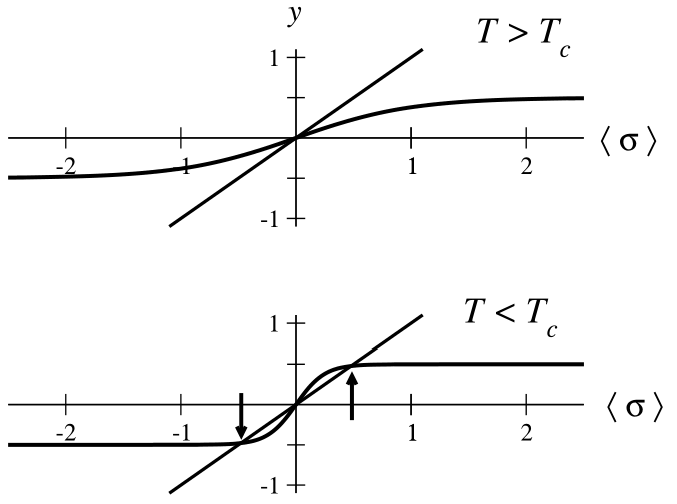
\includegraphics[width=.5\textwidth]{3e.png}
            \caption{教材图22.1,其中横坐标$\langle\sigma\rangle$就是本题中的$\langle S\rangle$.}
            \label{3e}
        \end{figure}
        \item[(f)] 当$S=1$,对一个特定的自旋其有效哈密顿量仍为
        \begin{align}
            \mathcal{H}=\bm{S}_i\cdot\left[-J\sum_j\langle\bm{S}_j\rangle+g\mu_B\bm{B}\right]=\bm{S}_i\cdot g\mu_B\bm{B}_{i,eff},
        \end{align}
        其中自旋$\bm{S}_i$感受到的有效磁场为
        \begin{align}
            g\mu_BB_{i,eff}=g\mu_B\bm{B}-J\sum_j\langle\bm{S}_j\rangle.
        \end{align}\\
        体系的配分函数为
        \begin{align}
            Z=\sum_{S=-1,0,+1}\exp(\beta E)=\exp(\beta g\mu_BB_{eff})+1+\exp(-\beta g\mu_BB_{eff}).
        \end{align}
        平均自旋为
        \begin{align}
            \langle S\rangle=\frac{-\exp(\beta g\mu_BB_{eff})+\exp(-\beta g\mu_BB_{eff})}{\exp(\beta g\mu_BB_{eff})+1+\exp(-\beta g\mu_BB_{eff})}=-\frac{2\sinh(\beta g\mu_BB_{eff})}{2\cosh(\beta g\mu_BB_{eff})+1}.
        \end{align}
        自洽方程为
        \begin{align}
            \langle S\rangle=-\frac{2\sinh[\beta(g\mu_BB-Jz\langle S\rangle]}{2\cosh[\beta(g\mu_BB-Jz\langle S\rangle)]+1}.
        \end{align}
        在高温下,自洽方程可以近似为
        \begin{gather}
            \langle S\rangle=-\frac{2}{3}\beta(g\mu_BB-Jz\langle S\rangle),\\
            \Longrightarrow\langle S\rangle=\frac{-\frac{2}{3}\beta g\mu_BB}{1-\frac{2}{3}\beta Jz}.
        \end{gather}
        体系的磁极化率为
        \begin{align}
            \chi=\mu_0\left.\frac{dM}{dB}\right\rvert_{B=0}=\mu_0\left.\frac{d(-Ng\mu_B\langle S\rangle)}{dB}\right\rvert_{B=0}=\frac{\frac{2}{3}\mu_0(g\mu_B)^2N}{k_BT-\frac{2}{3}Jz}=\frac{\frac{2}{3}\mu_0(g\mu_B)^2N}{k_B(T-T_c)},
        \end{align}
        其中临界温度
        \begin{align}
            T_c=\frac{2Jz}{3k_B}.
        \end{align}
    \end{enumerate}
\end{sol}

\begin{prob}[(22.4) Low-temperature Mean Field Theory]
    Consider the $S=1/2$ ferromagnet mean field calculation from Exercise 22.1. At zero temperature, the magnet is fully polarized.
    \begin{enumerate}
        \item[(a)] Calculate the magnetization in the very low temperature limit. Show that the deviation from fully polarized becomes exponentially small as $T$ goes to zero.
        \item[(b)$^*$] Now consider a spin $S$ ferromagnet. Determine the magnetization in the low $T$ limit. You can express your result conveniently in terms of the result of Exercise 22.3.
        \item[(c)$^*$] In fact this exponential behavior is not observed experimentally! The reason for this has to do with spinwaves, which are explored in Exercise 20.3, but are not included in mean field theory. Using some result from that exercise, determine (roughly) the low-temperature behavior of the magnetization of a ferromagnet.
    \end{enumerate}
\end{prob}
\begin{sol}
    \begin{enumerate}
        \item[(a)] 无外加磁场的情况下,自洽方程为
        \begin{align}
            \langle S\rangle=\frac{1}{2}\tanh(\beta Jz\langle S\rangle/2)
        \end{align}
        在低温极限下,自洽方程可以近似为
        \begin{align}
            \langle S\rangle=\frac{1}{2}\frac{1-\exp(-\beta Jz\langle S\rangle)}{1+\exp(-\beta Jz\langle S\rangle)}\approx\frac{1}{2}[1-\exp(-\beta Jz\langle S\rangle)]^2\approx\frac{1}{2}[1+2\exp(-\beta Jz\langle S\rangle)].
        \end{align}
        在低温下$\langle S\rangle\approx\frac{1}{2}$,故
        \begin{align}
            \langle S\rangle=\frac{1}{2}-\exp(-\beta Jz/2).
        \end{align}
        体系与完全极化之间的偏差呈现指数的形式,非常小.
        \item[(b)] 对于自旋为$S$的铁磁体,其在无外场下的自洽方程为
        \begin{align}
            \langle S\rangle=\frac{\sum_{S_z=-S,-S+1,\cdots,S-1,S}S_z\exp(-\beta J\langle S\rangle S_z)}{\sum_{S_z=-S,-S+1,\cdots,S-1,S}\exp(-\beta Jz\langle S \rangle S_z)}=\frac{\sum_{m=0,1,\cdots, 2S}(S-m)\exp(-\beta g\mu_B\langle S\rangle m)}{\sum_{m=0,1,\cdots,2S}\exp(-\beta g\mu_B\langle S\rangle m)}.
        \end{align}
        在低温极限下,自洽方程可以近似为
        \begin{align}
            \langle S\rangle\approx\left[\sum_{m=0,1,\cdots, 2S}(S-m)\exp(-\beta g\mu_B\langle S\rangle m)\right]\left[1-\sum_{m=1,2,\cdots,2S}\exp(-\beta g\mu_B\langle S\rangle m)\right]\approx S-\exp(\beta g\mu_B\langle S\rangle)
        \end{align}
        (先用$\frac{1}{1+x}\approx 1-x$,然后两个中括号相乘,仅保留零阶和一阶的指数线,舍去高阶的指数项)\\
        在低温下$\langle S\rangle=S$,故
        \begin{align}
            \langle S\rangle=S-\exp(\beta g\mu_B)
        \end{align}
        \item[(c)] 根据20.3题题干,铁磁体的自旋波的色散关系为
        \begin{align}
            \hbar\omega=g\mu_b\abs{B}+JS(6-2[\cos(k_xa)+\cos(k_ya)+\cos(k_za)]).
        \end{align}
        无外场的情况下,这一色散关系简化为
        \begin{align}
            \hbar\omega=4JS[\sin^2(k_xa/2)+\sin^2(k_ya/2)+\sin^2(k_za/2)].
        \end{align}
        对于波矢较小的情况,可以近似为
        \begin{align}
            \hbar\omega=JSa^2\abs{\bm{k}}^2.
        \end{align}
        自旋粒子的总个数为
        \begin{gather}
            \frac{V}{a^3}=\int\frac{d\bm{k}}{(2\pi)^3/V}=\int_0^{k_{max}}\frac{4\pi k^2\,dk}{(2\pi)^3}=\frac{4\pi k_{max}^3}{3(2\pi)^3}\\
            \Longrightarrow k_{max}=\frac{2\pi}{a}\left(\frac{3}{4\pi}\right)^{1/3}
        \end{gather}
        故平均自旋
        \begin{align}
            \langle S\rangle=\frac{a^3}{V}\int\frac{d\bm{k}}{(2\pi)^3/V}\frac{1}{e^{\beta JS^2a^2k^2}-1}=\frac{a^3}{2\pi^2}\int_0^{k_{max}}k^2\,dk\frac{1}{e^{\beta JS^2a^2k^2}-1}
        \end{align}
        由于晶格常数$a$很小,故$k_{max}$很大,上面的积分可以近似为积到正无穷,设$x^2=\beta JS^2a^2k^2$,上式可化为
        \begin{align}
            \langle S\rangle=\frac{1}{4\pi^2}\left(\frac{k_BT}{JS^2}\right)^{3/2}\int_0^{+\infty}dx\,\frac{\sqrt{x}}{e^{x}-1}\approx\frac{1}{4\pi^2}\left(\frac{k_BT}{JS^2}\right)^{3/2}\times 2.612\frac{\sqrt{\pi}}{2}.
        \end{align}
    \end{enumerate}
\end{sol}

\begin{prob}[(22.6) Correction to Mean Field$^*$]
    Consider the spin-$1/2$ Ising ferromagnet on a cubic lattice in $d$ dimensions. When we consider mean field theory, we treat exactly a single spin $\sigma_i$ and the $z=2d$ neighbors on each side will be considered to have an average spin $\langle\sigma\rangle$. The critical temperature you calculate should be $k_BT=Jz/4$.\\
    To improve on mean field theory, we can instead treat a block of two connected spins $\sigma_i$ and $\sigma_{i'}$, where the neighbors outside of this block are assumed to have the average spin $\langle\sigma\rangle$. Each of the spins in the block has $2d-1$ such average neighbors. Use this improved mean field theory to write a new equation for the critical temperature (it will be a transcendental equation). It this improved estimate of the critical temperature higher or lower than that calculated in the more simple mean-field method?
\end{prob}
\begin{sol}
    对于一对自旋,其总自旋用$\bm{\sigma}_i$表示,其哈密顿量为
    \begin{align}
        \mathcal{H}=\bm{\sigma}_i\cdot\left[-J\sum_j\langle\bm{\sigma}_j\rangle+g\mu_BB\right]+\mathcal{H}_1,
    \end{align}
    其中求和是针对与这对自旋相邻的自旋对,$\mathcal{H}_1$是这对自旋内部的自旋相互作用,
    \begin{align}
        \mathcal{H}_1=\left\{\begin{array}{ll}
            \frac{J}{4},&\sigma_i=0,\\
            -\frac{J}{4},&\sigma_i=\pm 1.
        \end{array}\right.
    \end{align}
    这一对自旋共有四种本征态
    \begin{align}
        (\uparrow,\uparrow),(\uparrow,\downarrow),(\downarrow,\uparrow),(\downarrow,\downarrow).
    \end{align}
    故体系的配分函数为
    \begin{align}
        Z=\exp[-\beta(J(z-1)\langle\sigma\rangle+g\mu_BB)+\beta J/4]+2\exp(-\beta J/4)+\exp[\beta(J(z-1)\langle\sigma\rangle+g\mu_BB)+\beta J/4]
    \end{align}
    自洽方程为
    \begin{align}
        \langle\sigma\rangle=\frac{\exp(\beta J/4)\sinh[\beta(J(z-1)\langle\sigma\rangle+g\mu_BB)]}{\exp(\beta J/4)\cosh[\beta(J(z-1)\langle\sigma\rangle+g\mu_BB)]+\exp(-\beta J/4)}.
    \end{align}
    在无外场的情况下,自洽方程为
    \begin{align}
        \langle\sigma\rangle=\frac{\exp(\beta J/4)\sinh[\beta J(z-1)\langle\sigma\rangle]}{\exp(\beta J/4)\cosh[\beta J(z-1)\langle\sigma\rangle]+\exp(-\beta J/4)}.
    \end{align}
    在$\langle\sigma\rangle=0$处,上式右边的斜率必须大于$1$才能保证上式有$\langle\sigma\rangle\neq 0$的解,即
    \begin{gather}
        \left.\frac{d}{d\langle\sigma\rangle}\frac{\exp(\beta J/4)\sinh[\beta J(z-1)\langle\sigma\rangle]}{\exp(\beta J/4)\cosh[\beta J(z-1)\langle\sigma\rangle]+\exp(-\beta J/4)}\right\rvert_{\langle\sigma\rangle=0}=\frac{[\beta J(z-1)][1+\exp(\beta J/2)]}{[\exp(\beta J/4)+\exp(-\beta J/4)]^2}>1,\\
        \Longrightarrow k_BT<\frac{J(z-1)}{4}\frac{\exp(\beta J/4)}{\exp(\beta J/4)+\exp(-\beta J/4)}.
    \end{gather}
    故临界温度
    \begin{align}
    T_c=\frac{J(z-1)}{4k_B}\frac{\exp(\beta J/4)}{\exp(\beta J/4)+\exp(-\beta J/4)}.
    \end{align}
    这样算出来的临界温度比未修正之前的更低.
\end{sol}

\begin{prob}[(23.1) Iteration Ferromagnetism]
    \begin{enumerate}
        \item[(a.i)]  Review 1: For a three-dimensional tight binding model on a cubic lattice, calculate the effective mass in terms of the hopping matrix element $t$ between nearest and the lattice constant $a$.
        \item[(a.ii)] Review 2: Assuming the density $n$ of electrons in this tight binding band is very low, one can view the electrons as being free electron with this effective mass $m^*$. For a system of spinless electrons show that the total energy per unit volume (at zero temperature) is given by
        \[
            E/V=nE_{min}+Cn^{5/3}
        \]
        where $E_{min}$ is the energy of the bottom of the band.
        \begin{itemize}
            \item[$\triangleright$] Calculate the constant $C$.
        \end{itemize}
        \item[(b)] Let the density of spin-up electrons be $n_{\uparrow}$ and the density of spin-down electrons be $n_{\downarrow}$. We can write these as
        \begin{gather}
            n_{\uparrow}=(n/2)(1+\alpha)\tag{23.6}\\
            n_{\downarrow}=(n/2)(1-\alpha)\tag{23.7}
        \end{gather}
        where the total net magnetization of the system is given by
        \[
            M=-\mu_bn\alpha
        \]
        Using the result of part (a), fixing the total density of electrons in the system $n$,
        \begin{itemize}
            \item[$\triangleright$] calculate the total energy of the system per volume as a function of $\alpha$.
            \item[$\triangleright$] Expand your result to fourth order in $\alpha$.
            \item[$\triangleright$] Show that $\alpha=0$ gives the lowest possible energy.
            \item[$\triangleright$] Argue that this remains true to all orders in $\alpha$
        \end{itemize}
        \item[(c)] Now consider adding a Hubbard interaction term
        \[
            H_{Hubbard}=U\sum_iN_{\uparrow}^iN_{\downarrow}^i
        \]
        with $U\leq 0$ where $N_{\sigma}^i$ is the number of electrons spin $\sigma$ on site $i$.\\
        Calculate the expectation value of this interaction term given that the up and down electrons form Fermi seas with densities $n_{\uparrow}$ and $n_{\downarrow}$ as given by Eqns. 23.6 and 23.7.
        \begin{itemize}
            \item[$\triangleright$] Write the energy in terms of $\alpha$.
        \end{itemize}
        \item[(d)] Adding together the kinetic energy calculated in part b with the interaction energy calculated in part c, determine the value of $U$ for which it is favorable for $\alpha$ to become non-zero.
        \begin{itemize}
            \item[$\triangleright$] For values of $U$ not too much bigger than this value, calculate the magnetization as a function of $U$.
            \item[$\triangleright$] Explain why this calculation is only an approximation.
        \end{itemize}
        \item[(e)] Consider now a two-dimensional tight binding model on a square lattice with a Hubbard interaction. How does this alter the result of part (b)?
    \end{enumerate}
\end{prob}
\begin{sol}
    \begin{enumerate}
        \item[(a.i)] 三维情况下紧束缚能谱为
        \begin{align}
            E=E_0-2t[\cos(k_xa)+\cos(k_ya)+\cos(k_za)]=E_0-2t[3-2\sin^2(k_xa/2)-2\sin^2(k_ya/2)-2\sin^2(k_za/2)].
        \end{align}
        在波矢较小的情况下,
        \begin{align}
            E\approx E_0-6t+ta^2(k_x^2+k_y^2+k_z^2)=E_0-6t+ta^2\abs{\bm{k}}^2=E_0-6t+\frac{\hbar^2\abs{\bm{k}}^2}{2m^*}.
        \end{align}
        故有效质量为
        \begin{align}
            m^*=\frac{\hbar^2}{2ta^2}.
        \end{align}
        \item[(a.ii)] 总原子数为
        \begin{align}
            N=\frac{V}{(2\pi)^3}\int_0^{k_f}d\bm{k}=\frac{V}{(2\pi)^3}\int_0^{k_f}4\pi k^2\,dk=\frac{V}{(2\pi)^3}\frac{4\pi k_f^3}{3},
        \end{align}
        从而费米波矢为
        \begin{align}
            k_f=(6\pi^2 n)^{1/3}.
        \end{align}
        电子的总动能为
        \begin{align}
            \nonumber E-N(E_0-6t)=&\frac{V}{(2\pi)^3}\int_0^{k_f}\frac{\hbar^2 k^2}{2m^*}\,d\bm{k}=\frac{V}{(2\pi)^3}\int_0^{k_f}\frac{\hbar^2k^2}{2m^*}4\pi k^2\,dk\\
            =&\frac{V}{(2\pi)^3}\frac{\hbar^2}{2m^*}\frac{4\pi k_f^5}{5}\propto n^{5/3}.
        \end{align}
        故单位体积中电子的总能量为
        \begin{align}
            E/V=nE_{min}+Cn^{5/3},
        \end{align}
        其中
        \begin{align}
            E_{min}=E_0-6t,
        \end{align}
        \begin{itemize}
            \item[$\triangleright$] 系数
            \begin{align}
                C=\frac{ta^2}{10\pi^2}(6\pi^2)^{5/3}.
            \end{align}
        \end{itemize}
        \item[(b)] 
        \begin{enumerate}
            \item[$\triangleright$] 单位体积中电子的总能量为
            \begin{align}
                \nonumber E/V=&nE_{min}+C[n_{\uparrow}^{5/3}+n_{\downarrow}^{5/3}]\\
                =&nE_{min}+C(n/2)^{5/3}[(1+\alpha)^{5/3}+(1-\alpha)^{5/3}].
            \end{align}
            \item[$\triangleright$] 将上式关于$\alpha$泰勒展开并保留到四阶项
            \begin{align}
                \nonumber E/V=&E_{min}n+2C(n/2)^{5/3}[1+(1/2!)(5/3)(2/3)\alpha^2+(1/4!)(5/3)(2/3)(-1/3)(-4/3)\alpha^4]\\
                =&E_{min}n+2C(n/2)^{5/3}[1+(5/9)\alpha^2+(5/243)\alpha^4].
            \end{align}
            \item[$\triangleright$] 当$\alpha=0$,可得单位体积中电子总能量的最低可能值
            \begin{align}
                (E/V)_{min}=E_{min}n+2C(n/2)^{5/3}
            \end{align}
            \item[$\triangleright$] 上面三个步骤对于任意高阶的近似都是适用的.
        \end{enumerate}
        \item[(c)] 
        \begin{itemize}
            \item[$\triangleright$] 晶体中的每个位点所占空间为$a^3$,所以每个位点的平均Hubbard相互作用能为$Ha^3/V$,每个位点上朝上的自旋数的期望值为$N_{\uparrow}=n_{\uparrow}a^3$,朝下的自旋数的期望值为$N_{\downarrow}=n_{\downarrow}a^3$,从而每个位点的平均Hubbard相互作用能为
            \begin{align}
                Ua^3/V=U(n_{\uparrow}a^3)(n_{\downarrow}a^3)=Ua^6(n/2)^2(1+\alpha)(1-\alpha)=Ua^3(n/2)^2(1-\alpha^2).
            \end{align}
            单位体积中Hubbard相互作用能的期望值为
            \begin{align}
                U/V=Ua^3(n/2)^2(1+\alpha)(1-\alpha)=Ua^3(n/2)^2(1-\alpha^2)
            \end{align}
        \end{itemize}
        \item[(d)] 单位体积中电子动能和Hubbard相互作用能量为
        \begin{align}
            E_{tot}/V=Ua^3(n/2)^2+\alpha^2[2C(5/9)(n/2)^{5/3}-Ua^3(n/2)^3]+\alpha^4[2C(n/2)^{5/3}(5/243)]
        \end{align}
        为了使$\alpha$可以为非零值,需要上面这一能量在$\alpha$较小的时候不随$\alpha$递增增加,故要求
        \begin{gather}
            2C(5/9)(n/2)^{5/3}-Ua^3(n/2)^3\leq 0,\\
            \Longrightarrow U\geq 2C(5/9)(n/2)^{-1/3}a^{-3}.
        \end{gather}
        \begin{itemize}
            \item[$\triangleright$] 对于不比上面这个值大很多的$U$,要使上面这个能量为最小值
            \begin{gather}
                \frac{d}{d\alpha}(E_{tot}/V)=2\alpha[2C(5/9)(n/2)^{5/3}-Ua^3(n/2)^3]+4\alpha^3[2C(n/2)^{5/3}(5/243)]=0,\\
                \Longrightarrow\alpha=\sqrt{-\frac{2C(5/9)(n/2)^{5/3}-Ua^3(n/2)^3}{4C(n/2)^{5/3}(5/243)}}.
            \end{gather}
            此时磁极化强度为
            \begin{align}
                M=-\mu_bn\alpha.
            \end{align}
            \item[$\triangleright$] 上面的这个计算结果只是一个近似值,因为我们已经略去了能量中关于$\alpha$的高于四阶的项.
        \end{itemize}
        \item[(e)] 在二维情况下,总原子数为
        \begin{align}
            N=\frac{A}{(2\pi)^2}\int_0^{k_f}d\bm{k}=\frac{A}{(2\pi)^3}\int_0^{k_f}2\pi k\,dk=\frac{A}{(2\pi)^2}\pi k_f^2,
        \end{align}
        其中$A$为总面积,从而费米波矢为
        \begin{align}
            k_f=\sqrt{4\pi n}.
        \end{align}
        电子的总动能为
        \begin{align}
            \nonumber E-NE_{min}=&\frac{A}{(2\pi)^2}\int_0^{k_f}\frac{\hbar^2k^2}{2m^*}d\bm{k}=\frac{A}{(2\pi)^2}\int_0^{k_f}\frac{\hbar^2k^2}{2m^*}2\pi k\,dk\\
            =&\frac{A}{(2\pi)^2}ta^2\frac{\pi}{2}(4\pi n)^2\propto n^2.
        \end{align}
        故单位面积中电子的总能量为
        \begin{align}
            E/A=nE_{min}+Cn^2,
        \end{align}
        其中系数
        \begin{align}
            C=2\pi ta^2.
        \end{align}
        若考虑电子的自旋方向,则
        \begin{align}
            \nonumber E/V=&nE_{min}+C[n_{\uparrow}^2+n_{\downarrow}^2]\\
            \nonumber=&nE_{min}+C(n/2)^2[(1+\alpha)^2+(1-\alpha)^2]\\
            =&nE_{min}+2C(n/2)^2[1+\alpha^2].
        \end{align}
    \end{enumerate}
\end{sol}
\end{document}